\documentclass[a4paper]{article}
\usepackage[latin9]{inputenc}
\usepackage[backref,pagebackref]{hyperref}
\makeatletter

% Test for a TeX4ht command:
\@ifundefined{HCode}{%
  % We are generating PDF, so allow to break down URL which is nicer
  % instead of ugly line overflows:
  \usepackage{breakurl}}{%
  % else we are generating HTML with TeX4ht, use plain url:
  \usepackage{url}}

\usepackage{xspace}
% \usepackage{makeidx}
\usepackage{wasysym}
\usepackage{graphicx}
\usepackage{xcolor}


%% For nice rendering of source codes:
\usepackage[hyper,procnames]{listings}
\lstset{extendedchars=true, language=C, basicstyle=\footnotesize\ttfamily, numbers=left,
  numberstyle=\tiny, stepnumber=2, numberfirstline=true, showspaces=true,
  showstringspaces=false, showtabs=true,
  tabsize=8, tab=\rightarrowfill, keywordstyle=\bf,
  stringstyle=\rmfamily, commentstyle=\rmfamily\itshape,
  index=[1][keywords],indexprocnames=true}

\sloppy

\newcommand{\LINK}[1]{\url{#1}\xspace}

\newcommand{\PipsOldWWW}{\LINK{http://www.cri.ensmp.fr/pips/}\xspace}
\newcommand{\PipsNewWWW}{\LINK{http://pips4u.org}\xspace}
\newcommand{\PipsDevGuidePDF}{\LINK{http://www.cri.ensmp.fr/pips/developer_guide.htdoc/developer_guide.pdf}}
\newcommand{\PipsDevGuideHTDOC}{\LINK{http://www.cri.ensmp.fr/pips/developer_guide.htdoc}}
\newcommand{\PipsAutotoolsGuidePDF}{\LINK{http://www.cri.ensmp.fr/pips/auto_pips.htdoc/auto_pips.pdf}}
\newcommand{\PipsAutotoolsGuideHTDOC}{\LINK{http://www.cri.ensmp.fr/pips/auto_pips.htdoc}}
\newcommand{\DoxygenSources}{\LINK{http://doxygen.pips.enstb.org/PIPS/graph}}

\title{{\Huge PIPS} \\ ~ \\ Tutorial to use PIPS with Eclipse \\ \normalsize{Rapport technique E-334}}

\author{
\begin{tabular}{rl}
  Nelson & \textsc{Lossing}
\end{tabular}\\
}

\date{January 10, 2014}

% \renewcommand{\indexname}{Index}
% \makeindex

% Number everything in the TOC:
\setcounter{secnumdepth}{10}
\setcounter{tocdepth}{10}

\begin{document}
\maketitle

\clearpage
\tableofcontents

\newpage

\section{Introduction}

This tutorial aims to explain how we can use Eclipse as IDE to work on PIPS. 
You can also read the PIPS developer guide 
\footnote{pdf version: \PipsDevGuidePDF \\ HTML version: \PipsDevGuideHTDOC} and 
the official web site of PIPS \PipsNewWWW for more information.

This document explains how we can configure the project linked with the SVN sources.
But also how to compile and to launch PIPS with Eclipse and so use the debugger provided by Eclipse.

This tutorial doesn't explain how to use Eclipse or the different possibilities offer by it.
(Switch between .c/.h, go to declaration, call Hierarchy, refactor, auto-completion, options during debug mode, etc.)

This tutorial and the screenshots are done with Eclipse JUNO version. 
So some little diffences can appear for other versions.

Most of the time, figures follow instructions. Think to turn the page to see them.


\section{Prerequisites}

Your Eclipse has to support C/C++ project.

You need to install \emph{subversive} in your Eclipse.
You can do this in \emph{``Help/Install New Software...''} and search svn to find subversive.

When you relaunch Eclipse after the first installation of \emph{subversive}, 
it will probably ask you to install a connector. You can install the lastest version of SVNKit.%For my part, I install SVNKit 1.7.8 (compatible for svn 1.7.x).


\section{Add the repositories of PIPS and their dependencies in Eclipse}
\label{sec:addSVNrepo}
The first thing to do is to add the SVN repositories of PIPS and their dependencies.


\begin{enumerate}
\item Switch to the \emph{SVN Repository Exploring}'s perspective. 
\begin{enumerate}
\item You can find this perspective in the perspective windows in menu \emph{``Windows/Open Perspective/Other...''} (right picture)
or button \emph{Open Perspective} (left picture).
\label{enum:it:choosePers}
\begin{center}
\noindent
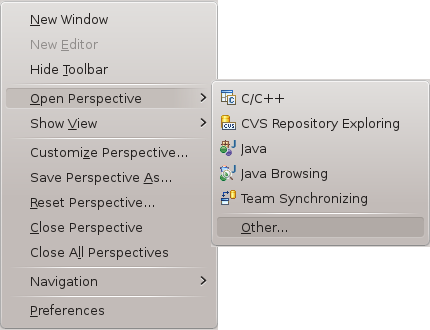
\includegraphics[scale=0.4]{eclipse/01-eclipseJUNO-openPerspective1.png}
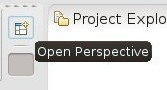
\includegraphics[scale=0.4]{eclipse/01-eclipseJUNO-openPerspective2.jpg}
\end{center}

\item Choose \emph{SVN Repository Exploring}. It will also add the shortcut in the \emph{Perspective view}.
\begin{center}
\noindent
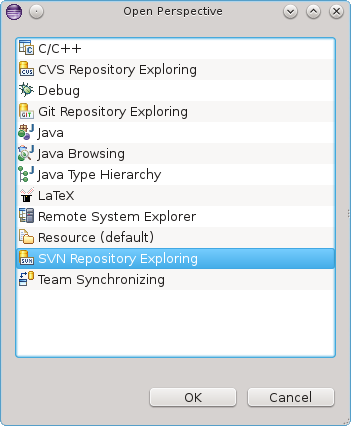
\includegraphics[scale=0.4]{eclipse/01-eclipseJUNO-openPerspective3.png}
\end{center}
\end{enumerate}


\item Add the repository location of PIPS \\(https://scm.cri.ensmp.fr/svn/pips/).
\begin{enumerate}
\item Open the \emph{New Repository Location} wizard.
\begin{center}
\noindent
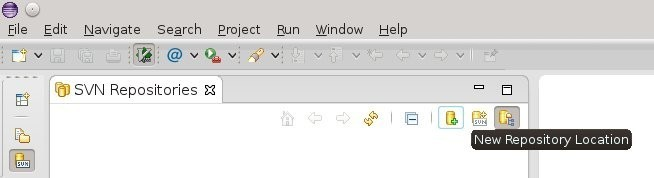
\includegraphics[scale=0.4]{eclipse/02-eclipseJUNO-newRepositories2.jpg}
\end{center}

\item Put the URL of PIPS https://scm.cri.ensmp.fr/svn/pips/ and your authentication login of PIPS. 
The authentication login of PIPS is optional. 
\begin{center}
\noindent
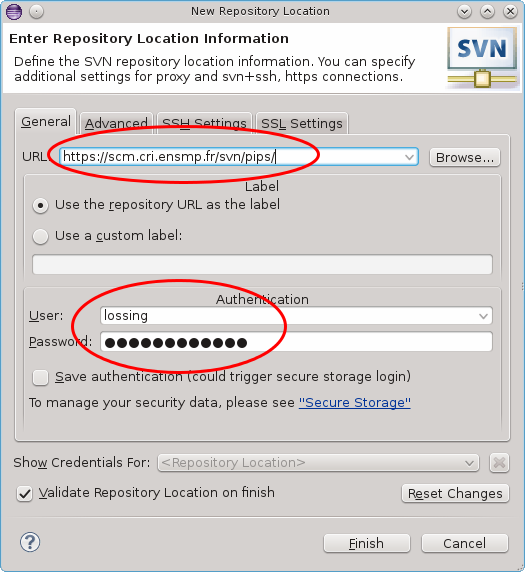
\includegraphics[scale=0.4]{eclipse/02-eclipseJUNO-newRepositories3.png}
\end{center}

\item click \emph{Finish}.
\end{enumerate}

\item Do the same for linear (https://scm.cri.ensmp.fr/svn/linear/) and Newgen (https://scm.cri.ensmp.fr/svn/newgen/).

You will normally have something like that at the end:
\begin{center}
\noindent
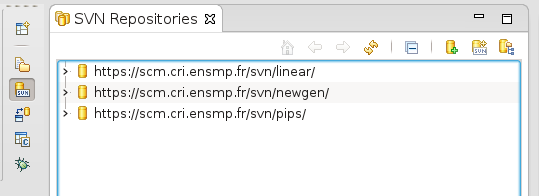
\includegraphics[scale=0.4]{eclipse/02-eclipseJUNO-newRepositories4.png}
\end{center}
\end{enumerate}


\section{Create the projects for PIPS}
\label{sec:makeproject}

You can now create a project that will be managed by Eclipse for PIPS under SVN.

\begin{enumerate}
\item Go back to the \emph{Ressource} Perspective or to the \emph{C/C++} Perspective \\
(see Sec~\ref{sec:addSVNrepo} step~\ref{enum:it:choosePers} to change the perspective).

\item Add a new SVN project for PIPS
(We want the project to be manage be svn).
\label{enum:it:newproject}
\begin{enumerate}
\item Create a new project (File/New/Project). 
\item Select a SVN project.
\begin{center}
\noindent
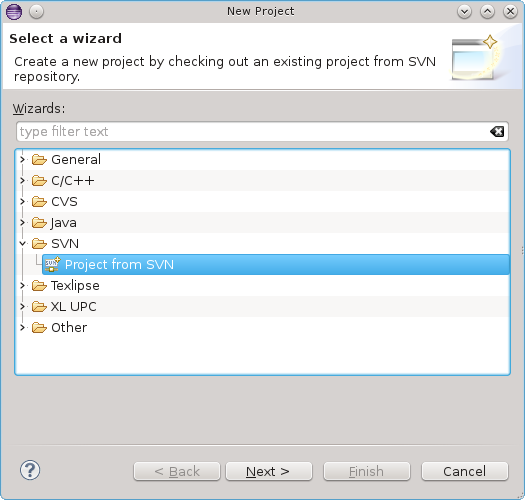
\includegraphics[scale=0.4]{eclipse/03-eclipseJUNO-newSVNProject1.png}
\end{center}

\item Select the PIPS URL.
\begin{center}
\noindent
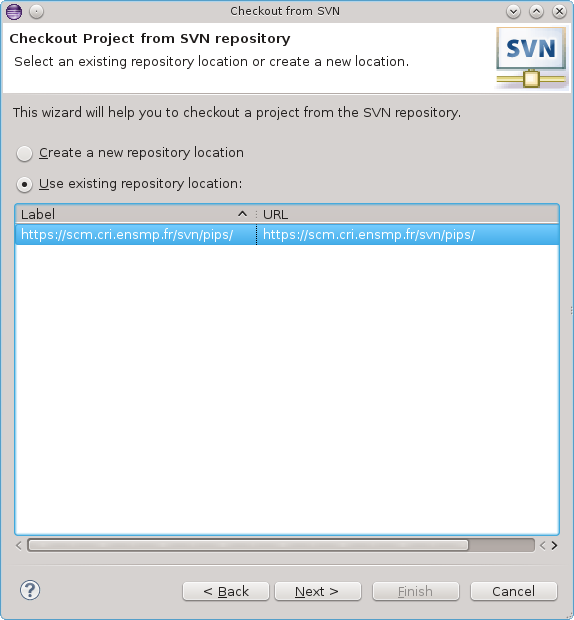
\includegraphics[scale=0.4]{eclipse/03-eclipseJUNO-newSVNProject2.png}
\end{center}

\item Select the trunk or your branch copy of the trunk. You can use \emph{``Browser...''} to help you select it. You can also choose an older revision if you want.

{\color{red}\textbf{\color{red} WARNING:} if you don't select the trunk or your specific branch, it will make a new project with all the depositories of PIPS (including trunk, all the branches and the tags).}
\begin{center}
\noindent$\!\!\!\!\!\!\!\!\!\!\!\!\!\!\!\!\!\!\!\!\!\!\!\!\!\!\!\!\!\!\!\!\!\!\!\!\!\!\!\!\!\!\!\!\!\!\!\!\!\!\!\!\!\!$
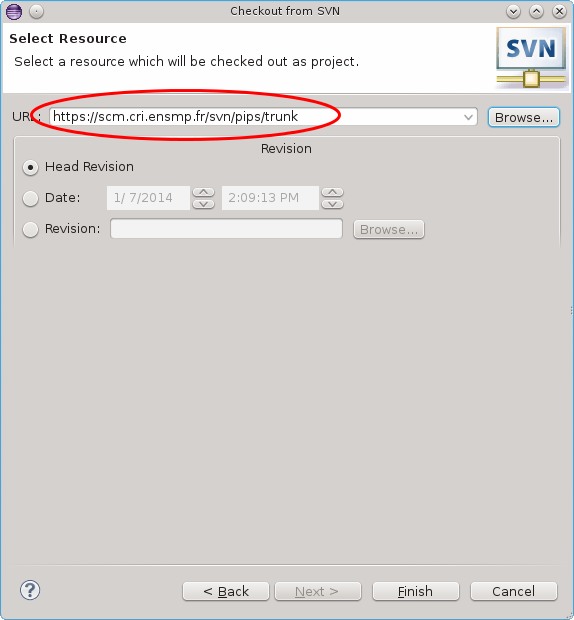
\includegraphics[scale=0.35]{eclipse/03-eclipseJUNO-newSVNProject3.png}
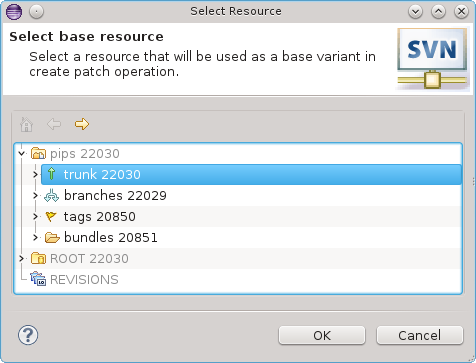
\includegraphics[scale=0.35]{eclipse/03-eclipseJUNO-newSVNProject4.png}
\end{center}

\item Click \emph{``Finish''}.

\item A new window appears. Choose \emph{Check out as a project with the name specified}.
\begin{center}
\noindent
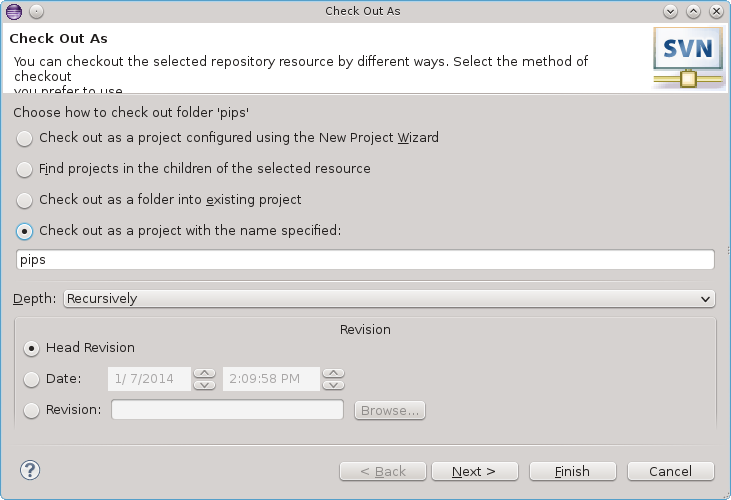
\includegraphics[scale=0.4]{eclipse/03-eclipseJUNO-newSVNProject5.png}
\end{center}

\item Click \emph{``Finish''}.
\end{enumerate}


\item Convert this new project into a C project
\begin{enumerate}
\item Right click on this new SVN project and choose \emph{``New/Convert to C/C++ Project (Add C/C++ Nature)''}
\begin{center}
\noindent
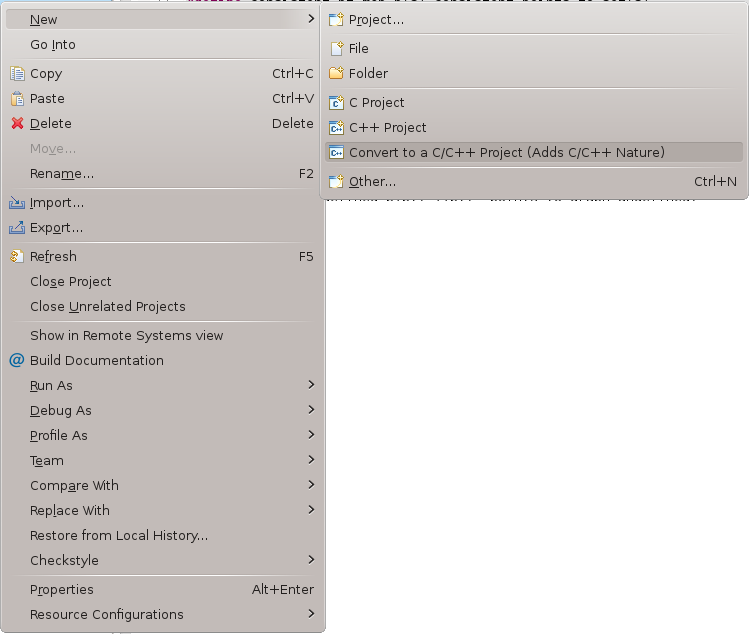
\includegraphics[scale=0.4]{eclipse/04-eclipseJUNO-convertToCproject1.png}
\end{center}

\item Choose to convert into a C project.\\
%(For project options, I choose a Makefile project and LINUX GCC like toolchains, 
%but I'm not sure if it's necessary or if an Executable is not better.)\\
\textbf{Note:} you can convert many projects in one step, if your SVN project is added as Candidate for conversion (empty in the screenshot)
\begin{center}
\noindent
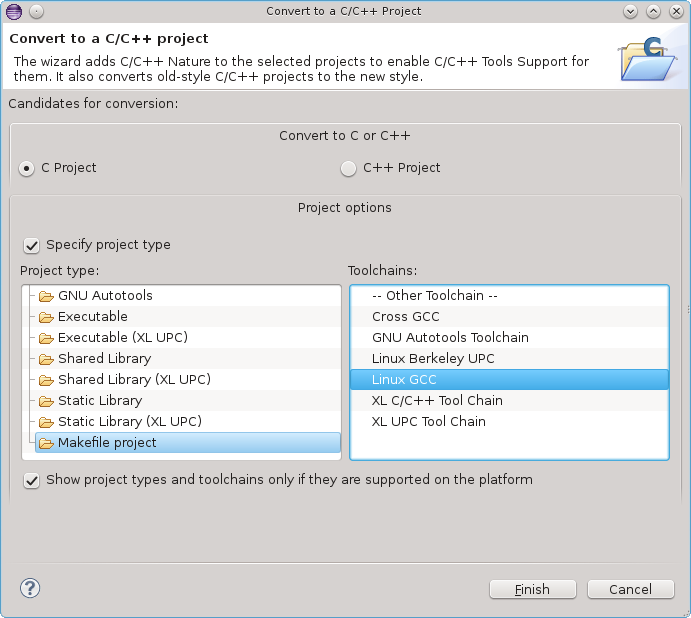
\includegraphics[scale=0.4]{eclipse/04-eclipseJUNO-convertToCproject2.png}
\end{center}

\item Click \emph{``Finish''}.
\end{enumerate}

\item Do the same for linear and newgen and your personal version of PIPS (in your branch). (Sec~\ref{sec:makeproject} step~\ref{enum:it:newproject}.)
\end{enumerate}



\section{Configure your projects}
\label{sec:confProject}

\begin{enumerate}
\item Add the \emph{include} path for the different dependencies.
\label{enum:it:addsymb}

For this purpose you can see the developer\_guide part \textbf{Section 3.2.2 Missing includes}.
In summary, these configurations are done in the property project, menu ``C/C++ General'', submenu ``Paths and Symbols'', ``Include'' tab.

Without these includes, you won't be able to use the power of Eclipse.

Some folders are only present after a first compilation (the \textit{include} folders). 
But you can put them manually into the configuration without problems.

List of includes for the different projects:
\begin{enumerate}
\item \textbf{newgen} needs: /newgen/include
\item \textbf{linear} needs: /linear/inlcude AND include from {\color{red} polylib}
\item \textbf{PIPS} needs:   /newgen/include, /linear/inlcude and /pips/include
\end{enumerate}

\textbf{Note:} For polylib, when you add a path choose ``File System...'' and find where you install polylib (into extern).

\textbf{Note:} If you want to compile in consol mode, I recommand to copy the extern folder make by the standard version installation of PIPS \footnote{\LINK{http://pips4u.org/copy_of_getting-pips/building-and-installing-pips-from svn}}.

\item Modify the \emph{Path} Environnement to add pipsrc. 
It corresponds to the path added with pipsrc.sh.
\label{enum:it:addpath}

\begin{enumerate}
\item Open the properties of your pips project \\
\emph{Alt+Enter} or right-click on your pips project or \emph{File/Properties}.
\begin{center}
\noindent
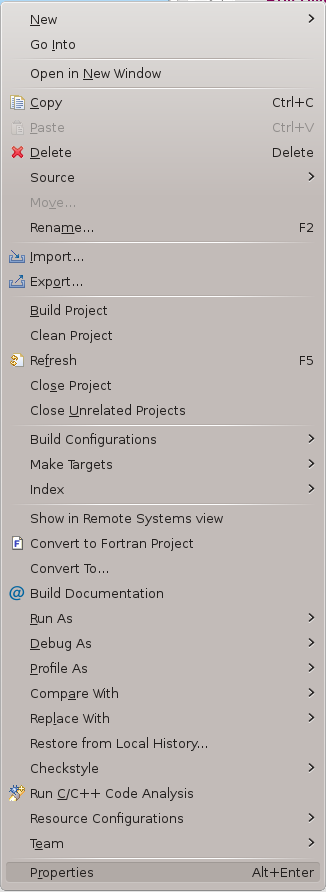
\includegraphics[scale=0.4]{eclipse/05-eclipseJUNO-addPath1.png}
\end{center}

\item Select \emph{C/C++ Build/Environment}. Click Add.

\noindent$\!\!\!\!\!\!\!\!\!\!\!\!\!\!\!\!\!\!\!\!\!\!\!\!\!\!\!\!\!\!\!\!\!\!\!\!\!\!\!\!\!\!\!\!\!\!\!\!\!$
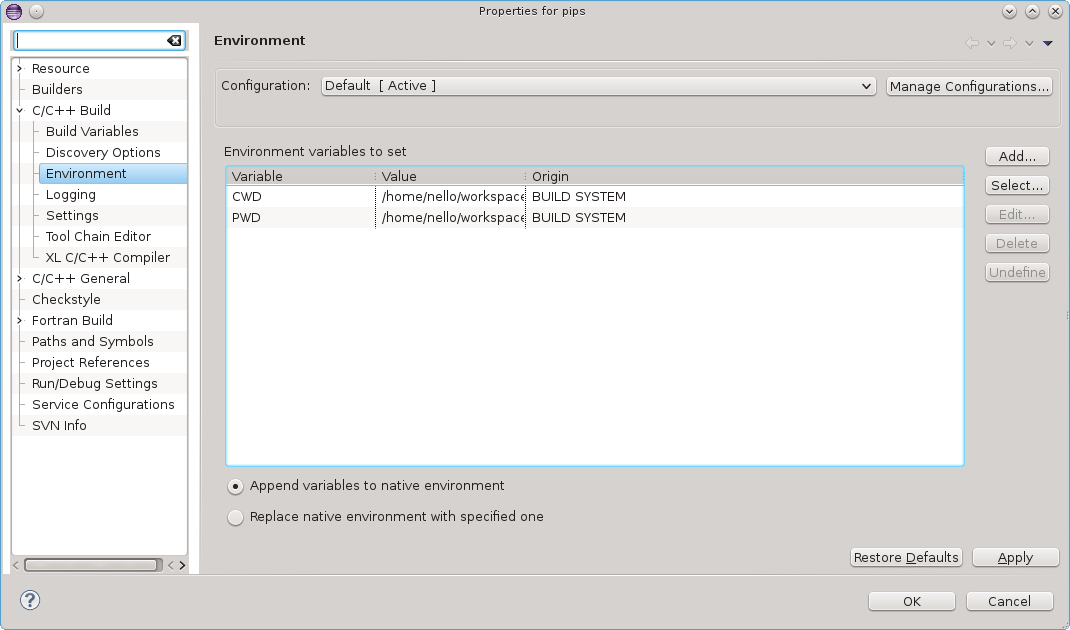
\includegraphics[scale=0.4]{eclipse/05-eclipseJUNO-addPath2.png}

\item Add the variable \textbf{\emph{PATH}} with the value \\\textbf{\emph{\$\{PATH\}:\\\$\{WorkspaceDirPath\}/pips/bin:\\\$\{WorkspaceDirPath\}/pips/utils:\\\$\{WorkspaceDirPath\}/newgen/bin}}

Replace \emph{pips} by the name of your pips project if it needs.
\begin{center}
\noindent
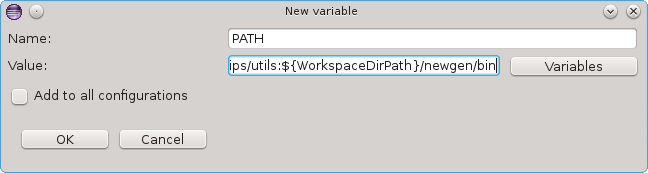
\includegraphics[scale=0.4]{eclipse/05-eclipseJUNO-addPath3.png}
\end{center}

\item \emph{Apply} your modfication and click \emph{OK}.

\noindent$\!\!\!\!\!\!\!\!\!\!\!\!\!\!\!\!\!\!\!\!\!\!\!\!\!\!\!\!\!\!\!\!\!\!\!\!\!\!\!\!\!\!\!\!\!\!\!\!\!$
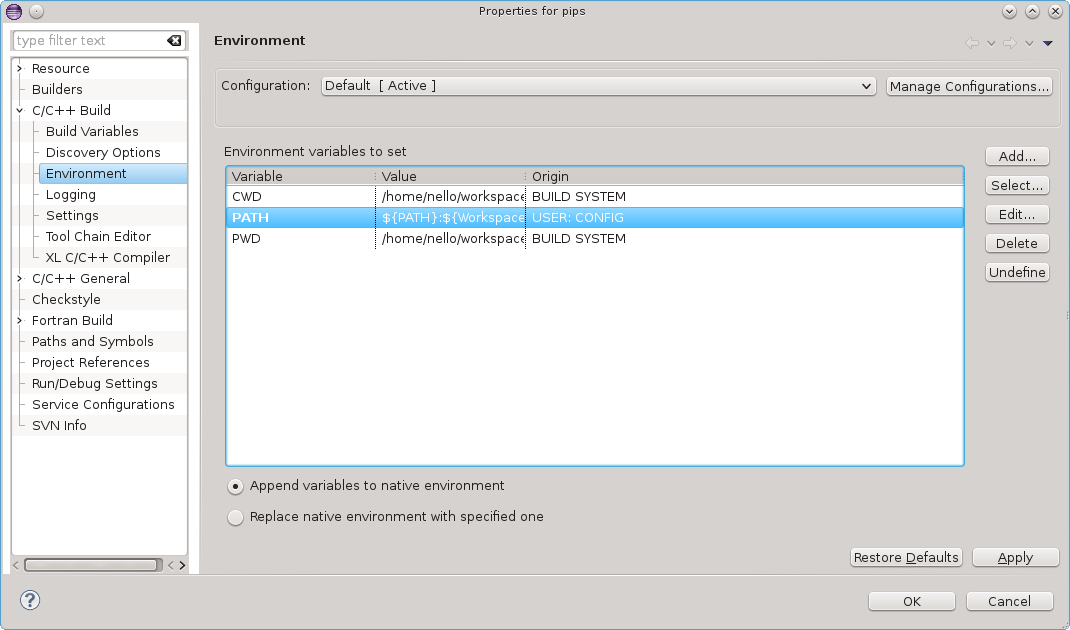
\includegraphics[scale=0.4]{eclipse/05-eclipseJUNO-addPath4.png}
\end{enumerate}
\end{enumerate}


After this configuration has been done, you can use PIPS in Eclipse.

\newpage

\section{How can we compile PIPS with Eclipse?}

Compilation corresponds to build your project in Eclipse.

If you want to use the binary make by the compilation for debug, you have to modify optimization compilation, see \ref{sec:faq:randomdebug}.

For the first compilation, you have to build \emph{newgen} and \emph{linear} before the \emph{pips} project.

\begin{enumerate}
\item Right click on the project you want to compile and choose build:
\begin{center}
\noindent
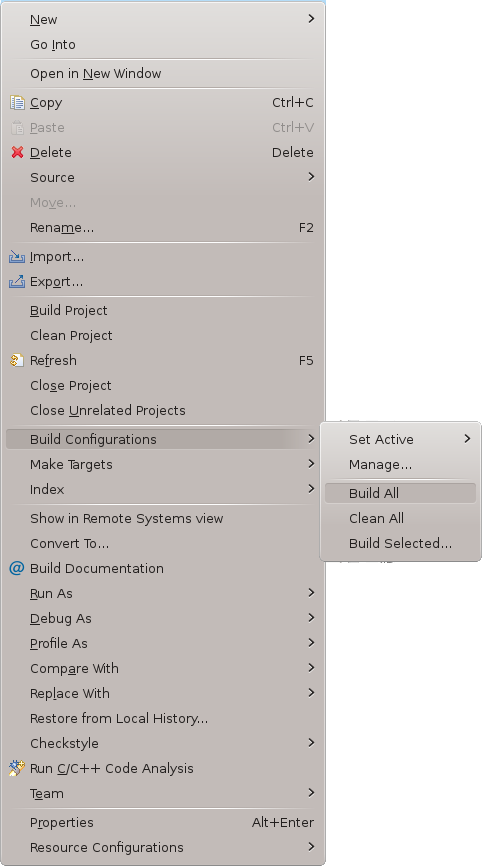
\includegraphics[scale=0.4]{eclipse/06-eclipseJUNO-build1.png}
\end{center}

\item You can also select your project and use the shortcut in the C/C++ perspective:
\begin{center}
\noindent
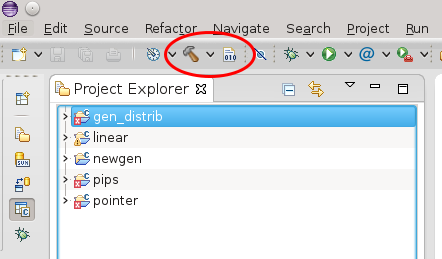
\includegraphics[scale=0.4]{eclipse/06-eclipseJUNO-build2.png}
\end{center}
\end{enumerate}


\section{How can we debug PIPS with Eclipse?}

For this purpose, you will need to set a debug configuration.

\begin{enumerate}
\item Right click on your PIPS project, and choose \emph{``Debug As/Debug Configuration''}. 
In C/C++ perspective you can use the arrow near the shortcut.
\begin{center}
\noindent
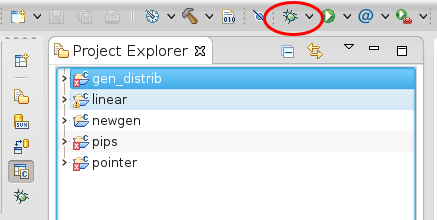
\includegraphics[scale=0.4]{eclipse/07-eclipseJUNO-debug1.png}
\end{center}

\item Select C/C+++ Application and click on \emph{``New''}.
\begin{center}
\noindent
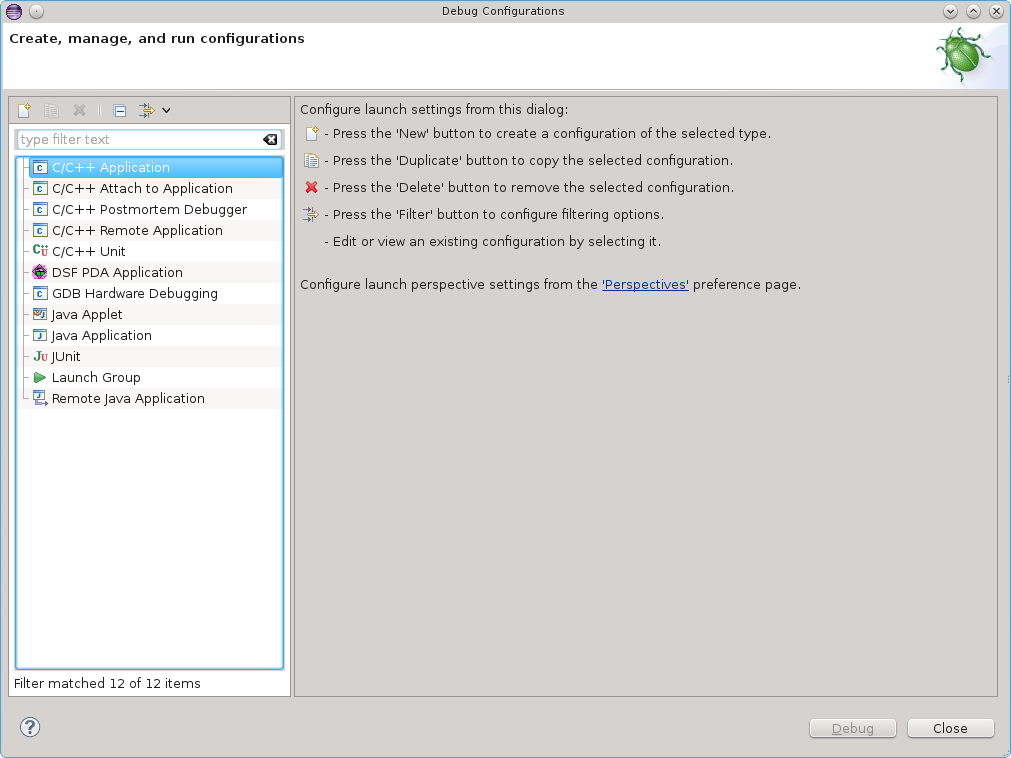
\includegraphics[scale=0.35]{eclipse/07-eclipseJUNO-debug2.png}
\end{center}

\item Click on \emph{``Search Project''} to define what you want to launch.
\begin{center}
\noindent
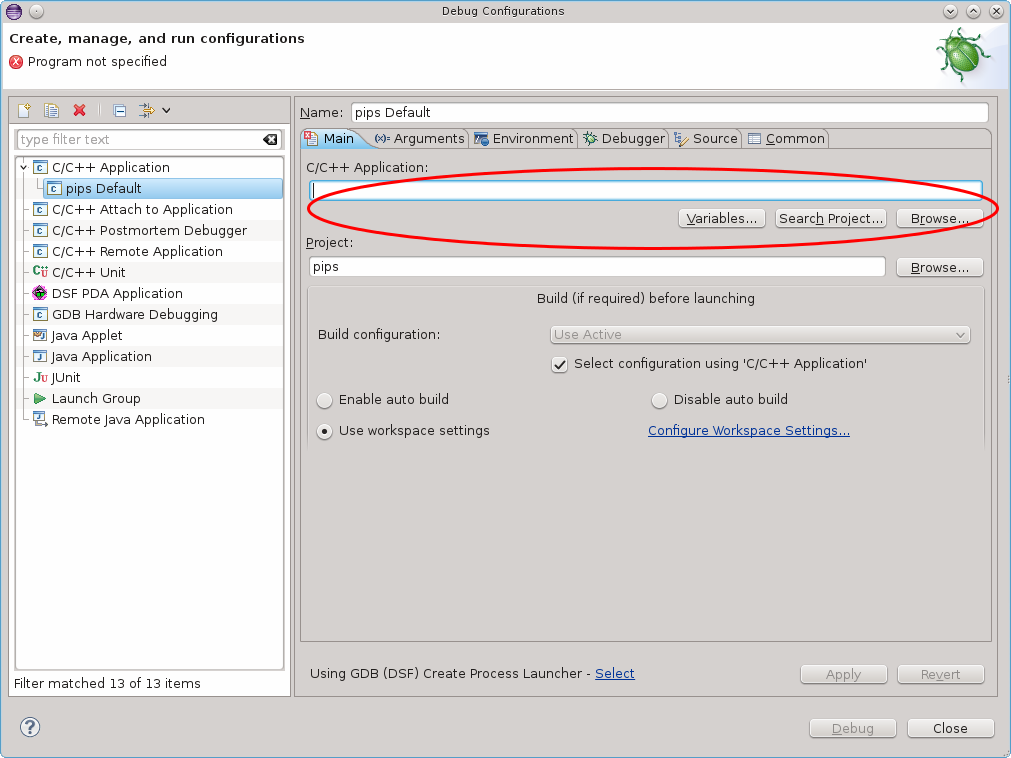
\includegraphics[scale=0.4]{eclipse/07-eclipseJUNO-debug3.png}
\end{center}

\item Select \emph{tpips} and the binary corresponding.
\begin{center}
\noindent
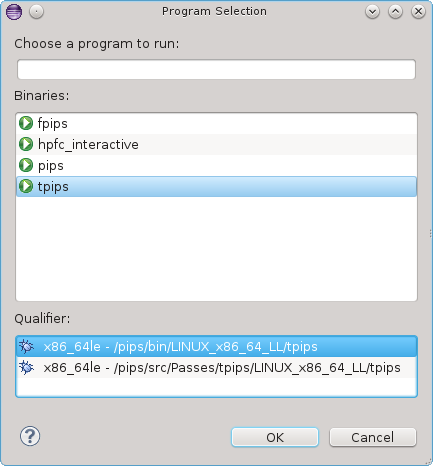
\includegraphics[scale=0.4]{eclipse/07-eclipseJUNO-debug4.png}
\end{center}

\item Configure the arguments to send your tpips file to execute. 
Without them, you have to write yourself the different instructions.
\begin{center}
\noindent
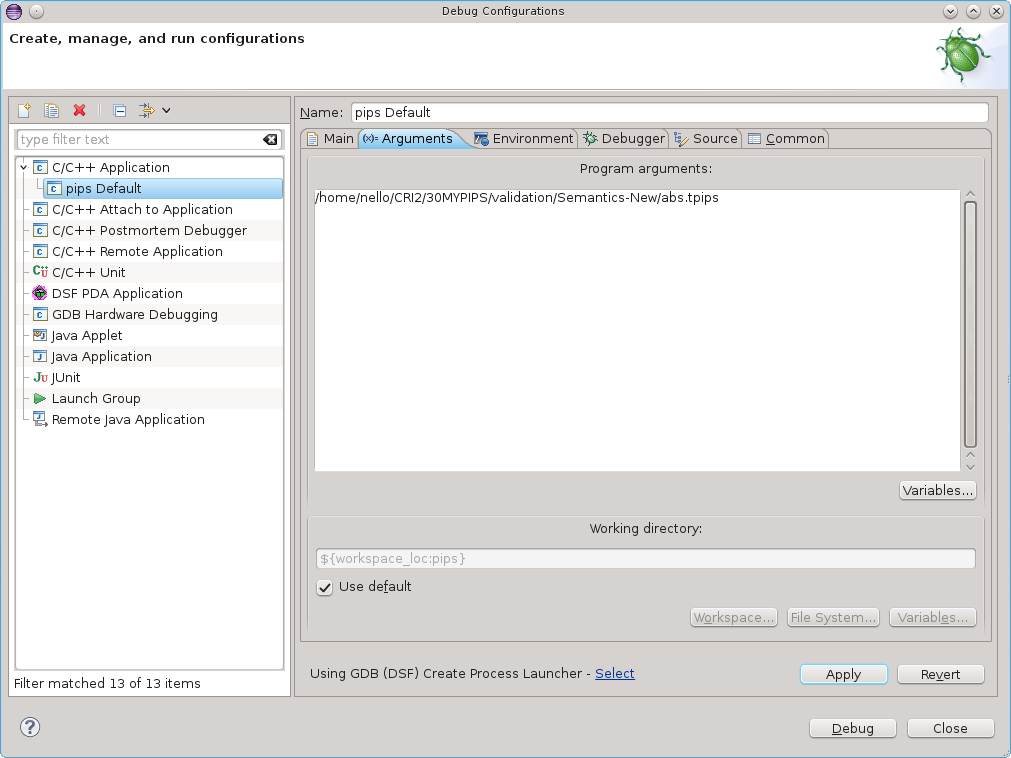
\includegraphics[scale=0.4]{eclipse/07-eclipseJUNO-debug5.png}
\end{center}

\item Click on \emph{``Apply''}, Click on \emph{``Debug''}

\item Enjoy your debug with Eclipse.

\end{enumerate}

\newpage

\section{FAQ}

\subsection{Why do I have many red-underline words?}

When a word is underlined by Eclipse, it's mean that it detects a problem.

If the problem say ``xxx cannot be resolved'', you have to rebuild the index.

First, you have to configure your ``Paths and Symbols'' (see step \ref{enum:it:addsymb} in Sec. \ref{sec:confProject}), if it's not already done.

After that, right click on your project, select Index, and click on \emph{``Rebuild''}.

The problem must be resolved.


\subsection{Why can I only launch the debug for tpips only once?}

You have to configure the PATH environnement variable, see step \ref{enum:it:addpath} in Sec. \ref{sec:confProject} Configure your project.

% Eclipse can't execute the command {\em delete} of the tpips file. I don't know why for that moment.
% 
% So you have to delete it manually. The data folder is located in the workspace of Eclipse in the project that launch tpips.
% 
% After delete it, you can relaucnh your tpips.


\subsection{Why debug step go randomly top and down?}
\label{sec:faq:randomdebug}

You have to compile without optimization options. The same thing will happens with gdb if the compilation is not configure.

In the file \emph{makes/gnu-stuff.mk}, put -O0 instead of -O2.



\subsection{How can I ask Eclipse to not recompil before launch debug?}

Because of the complexity of the PIPS project, Eclipse seems to think that there is a modification into this project when it's not the case.
So we have to disable this option.

In \emph{Windows/Preferences}, select \emph{Run/Debug} menu, \emph{Launching} submenu. Uncheck \emph{Build (if required) before launching}.
\begin{center}
\noindent
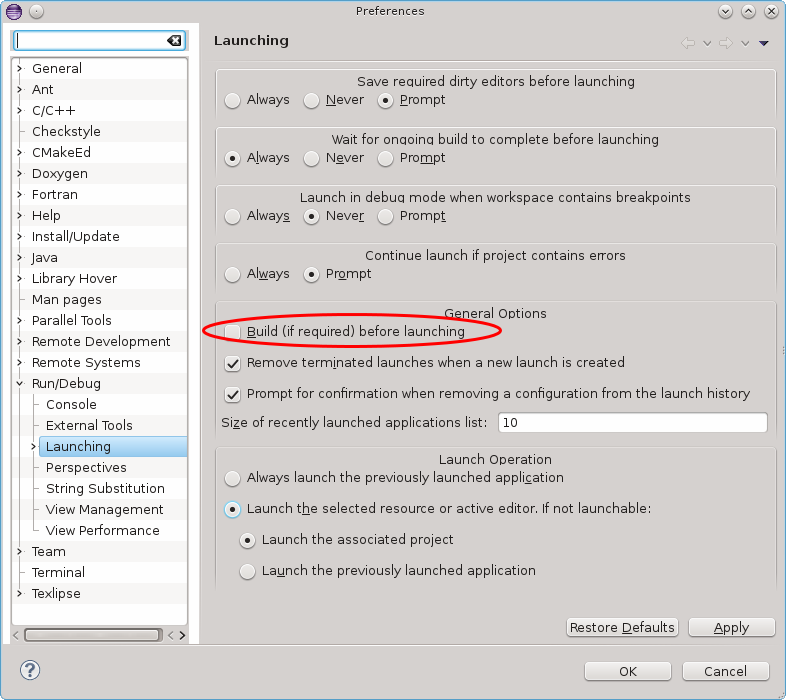
\includegraphics[scale=0.4]{eclipse/09-eclipseJUNO-launchConfig.png}
\end{center}

\subsection{How can I use SVN in Eclipse?}

You can open the \emph{Team Synchronizing} perspective for this purpose.
You can also right click on a folder or file and look the different possibilities of \emph{Team}.
\begin{center}
\noindent
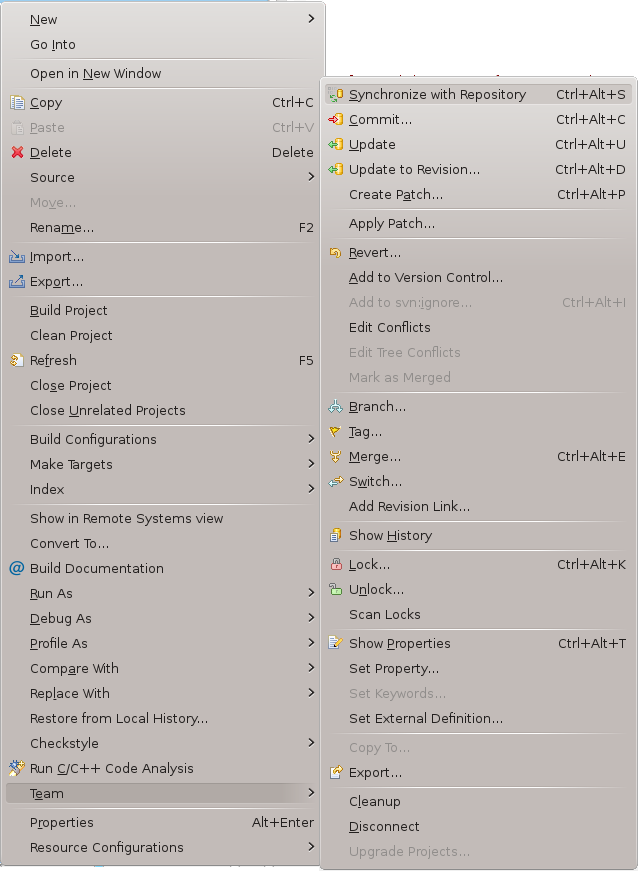
\includegraphics[scale=0.4]{eclipse/08-eclipseJUNO-synchronization-with-eclipse.png}
\end{center}

{\color{red}\textbf{\color{red} WARNING:} Take care to not commit the Eclipse settings or some files coming from compilation especially in the trunk.}

%(I do not try to merge, branch or copy from or to the trunk with Eclipse. I prefer use the console for this purpose, all the explanations are done in the developer\_guide.)

\newpage

% 
% {\small
% \bibliographystyle{plain}
% \bibliography{developer_guide}
% }
% 
% \printindex

\end{document}
